\documentclass{article}\usepackage[]{graphicx}\usepackage[]{color}
%% maxwidth is the original width if it is less than linewidth
%% otherwise use linewidth (to make sure the graphics do not exceed the margin)
\makeatletter
\def\maxwidth{ %
  \ifdim\Gin@nat@width>\linewidth
    \linewidth
  \else
    \Gin@nat@width
  \fi
}
\makeatother

\definecolor{fgcolor}{rgb}{0.345, 0.345, 0.345}
\newcommand{\hlnum}[1]{\textcolor[rgb]{0.686,0.059,0.569}{#1}}%
\newcommand{\hlstr}[1]{\textcolor[rgb]{0.192,0.494,0.8}{#1}}%
\newcommand{\hlcom}[1]{\textcolor[rgb]{0.678,0.584,0.686}{\textit{#1}}}%
\newcommand{\hlopt}[1]{\textcolor[rgb]{0,0,0}{#1}}%
\newcommand{\hlstd}[1]{\textcolor[rgb]{0.345,0.345,0.345}{#1}}%
\newcommand{\hlkwa}[1]{\textcolor[rgb]{0.161,0.373,0.58}{\textbf{#1}}}%
\newcommand{\hlkwb}[1]{\textcolor[rgb]{0.69,0.353,0.396}{#1}}%
\newcommand{\hlkwc}[1]{\textcolor[rgb]{0.333,0.667,0.333}{#1}}%
\newcommand{\hlkwd}[1]{\textcolor[rgb]{0.737,0.353,0.396}{\textbf{#1}}}%
\let\hlipl\hlkwb

\usepackage{framed}
\makeatletter
\newenvironment{kframe}{%
 \def\at@end@of@kframe{}%
 \ifinner\ifhmode%
  \def\at@end@of@kframe{\end{minipage}}%
  \begin{minipage}{\columnwidth}%
 \fi\fi%
 \def\FrameCommand##1{\hskip\@totalleftmargin \hskip-\fboxsep
 \colorbox{shadecolor}{##1}\hskip-\fboxsep
     % There is no \\@totalrightmargin, so:
     \hskip-\linewidth \hskip-\@totalleftmargin \hskip\columnwidth}%
 \MakeFramed {\advance\hsize-\width
   \@totalleftmargin\z@ \linewidth\hsize
   \@setminipage}}%
 {\par\unskip\endMakeFramed%
 \at@end@of@kframe}
\makeatother

\definecolor{shadecolor}{rgb}{.97, .97, .97}
\definecolor{messagecolor}{rgb}{0, 0, 0}
\definecolor{warningcolor}{rgb}{1, 0, 1}
\definecolor{errorcolor}{rgb}{1, 0, 0}
\newenvironment{knitrout}{}{} % an empty environment to be redefined in TeX

\usepackage{alltt}
\usepackage[letterpaper, portrait, margin=1in]{geometry}
\IfFileExists{upquote.sty}{\usepackage{upquote}}{}
\begin{document}

\title{STAT 243 Final Project}
\author{Ming Qiu, Junyuan Gao, Jeffrey Kwarsick, Titouan Jehl}
\date{December 14, 2017}
\maketitle

\section{Final Project Location}
Our Genetic Algorithm (GA) Package is located on Ming Qiu’s github. The account name is
\textbf{carslawbroccoli}.

\section{Skeleton of the Genetic Algorithm}
To implement the genetic algorithm, we chose to break the algorithm into independent blocks so
each of us could work separately. To realize those standalone blocks we first consider two parts
that are separable the initialization and the loop. Initialisation should create the first generation
from the data provided by the user and the number of individual per generation. On the other
hand the loop can still be broken into subblocks. We decided to implement 5 methods:

\begin{itemize}
  
  \item a ‘training‘ method that takes as input a candidate with his information, data, a model to fit
  and fitness function. This method fits the model on the data with respect to the candidate
  genetic information. It then outputs the fitness value of this candidate. This method dealing
  with only one candidate as a time, it enables us to later parallelize the update of a generation
  by running this method on different cores.
  
  \item a ‘select parent‘ method that takes as input the vector of fitness values of the candidate of
  the current generation as well as all the way to select the parents - with/without replacement,
  tournament, etc. This method selects pairs of parents with respect to the fitness values of the
  candidate. It returns a list of pairs of parents that will breed to create the next generation
  
  \item a ‘breeding‘ method that takes as input the pairs of parents, and the input needed to chose the
  breeding technique (number of crossover points etc.). This methods create the candidates of
  the next generation. This method does not implement the mutation. Note that this method
  could have been split in a smaller block on which we could have parallelize a loop. The
  output of this method is the binary dataframe representing the genetic information of the
  next generation
  
  \item a ‘mutation‘ method that takes as input the new generation and the rate of mutation to
  modify the genetic information randomly and output the new generation post mutations
  
  \item a ‘get model‘ method that returns for a given candidate the model that has been fitted on it

\end{itemize}

Each of these methods are completely stand alone and can be tested without the rest of the method.
However, provided the right comments to standardize the input and the output so assembling the
blocks doesn’t raise errors, this skeleton enables the team to separately implement the algorithm
efficiently.

\section{Collaborator Contributions}

\subsection{Ming Qiu's Contribution}
Ming Qiu worked on the select.R function that handles the iterations for the genetic algorithm as
well as the training function.  She also worked to implement plotting features for our algorithm with the \emph{get\_model()} function.  Lastly, she worked to debug the package as a whole to run more efficiently. She also worked on the \emph{get_model()} function.

\subsection{Junyuan Gao's Contribution}
Junyuan Gao worked on the formal testing for the completed algorithm, checking to ensure thatproper inputs for each function in our algorithm were able to handle improper inputs. He also worked on writing the breeding function (crossover and mutation included within the breeding function).

\subsection{Jeffrey Kwarsick's Contribution}
Jeffrey Kwarsick worked on the \emph{select\_parents()} function. He was also responsible for building
the package and making sure it carried the proper structure.  He ensured that it was able to be installed through github and tested.  Lastly, he prepared all of the documentation within the package itself.

\subsection{Titouan Jehl's Contribution}
Titouan designed the skeleton. He coded the skeleton of the ‘utils.R‘ file so the whole group could be on the same page about the data type of the inputs and outputs. To do so I adopted the Google style of comment for each method.

\section{Testing}
We conducted testing on all of the inputs for all functions in our package and confirmed that if an invalid input was entered, that the code would properly handle the error and not execute. In addition to testing all of the outputs, all the functions were also tested independently. Below is an itemized list of how each function within our algorithm was tested.

\begin{itemize}
  \item training
  \begin{itemize}
    \item The algorithm works with both lm() and glm().
    \item That the algorithm works with both AIC and BIC for fitness functions.
    \item That the output vector of the training function is non-zero and correctly outputs all
          fitness values for candidate chromosomes.
  \end{itemize}
  \item select_parents
  \begin{itemize}
    \item The function produces correct length of parent pairs for breeding
    \item That each call of select parents() produces a different set of parent pairs for breeding.
    \item If either selection mechanism is called, the same number of parent pairs (based on the
          number of input parents) is the same.
  \end{itemize}
  \item breed
  \begin{itemize}
    \item That the output is a data frame of the correct (P x c) dimension
    \item Everytime repeated crossover and mutation will produce different new generations
    \item That the generation gap can only be between (0,1]
  \end{itemize}
  \item get\_model -- output is the same class as the training method
  \item select -- integration test of the function, checking all inputs
\end{itemize}

\section{Example}
Below is an example for fitting using an R dataset \textbf{mtcars}, with the dependent variable being \textbf{mpg}.

\begin{knitrout}
\definecolor{shadecolor}{rgb}{0.969, 0.969, 0.969}\color{fgcolor}\begin{kframe}
\begin{alltt}
\hlkwd{library}\hlstd{(}\hlstr{'GA'}\hlstd{)}
\hlkwd{library}\hlstd{(}\hlstr{'ggplot2'}\hlstd{)}

\hlkwd{select}\hlstd{(mtcars,} \hlstr{"mpg"}\hlstd{,} \hlkwc{plot.return} \hlstd{=} \hlnum{TRUE}\hlstd{)}
\end{alltt}
\end{kframe}
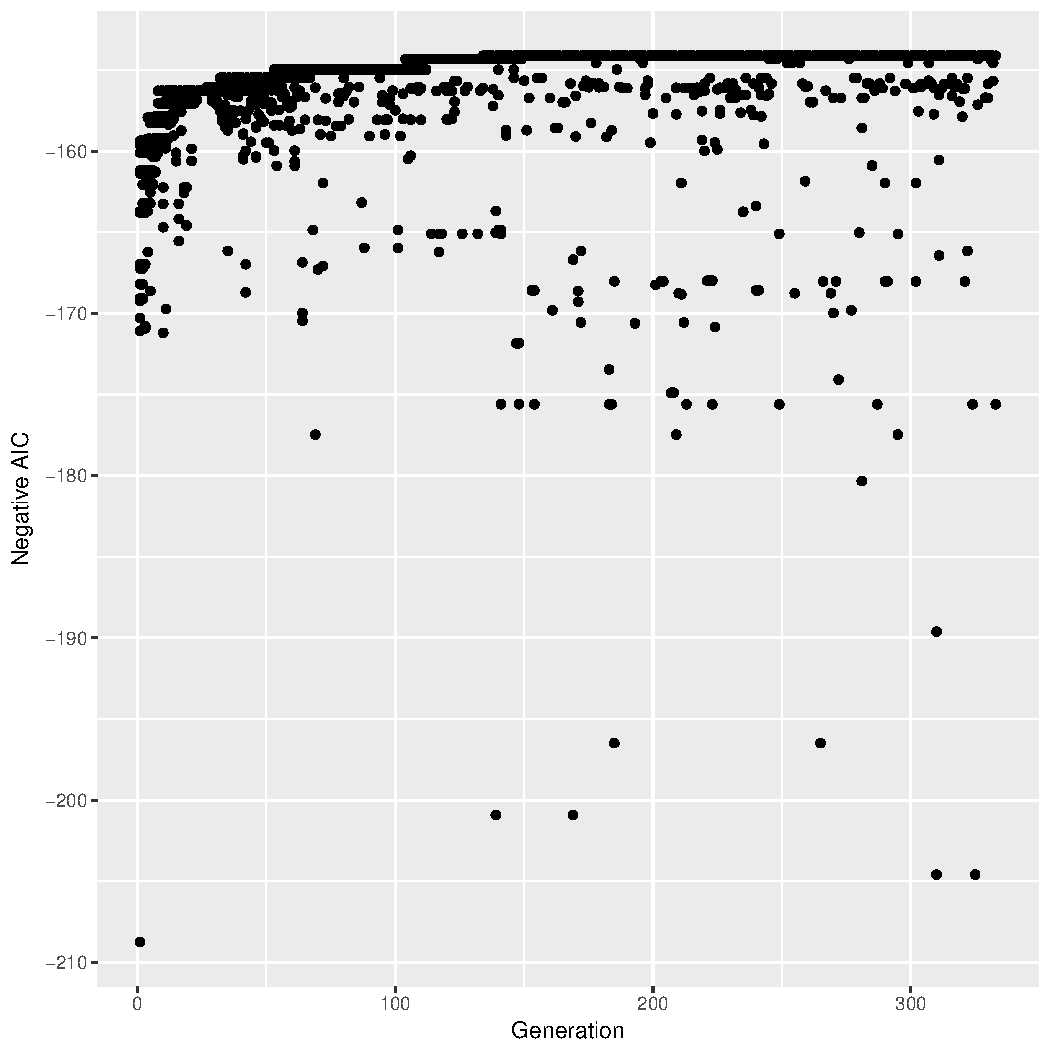
\includegraphics[width=\maxwidth]{figure/unnamed-chunk-1-1} 
\begin{kframe}\begin{verbatim}
## $count
## [1] 333
## 
## $model
## 
## Call:
## method(formula = fmla, data = X)
## 
## Coefficients:
## (Intercept)           wt         qsec           am  
##       9.618       -3.917        1.226        2.936  
## 
## 
## $fitness_value
## [1] 154.1194
## 
## $plot
\end{verbatim}
\end{kframe}
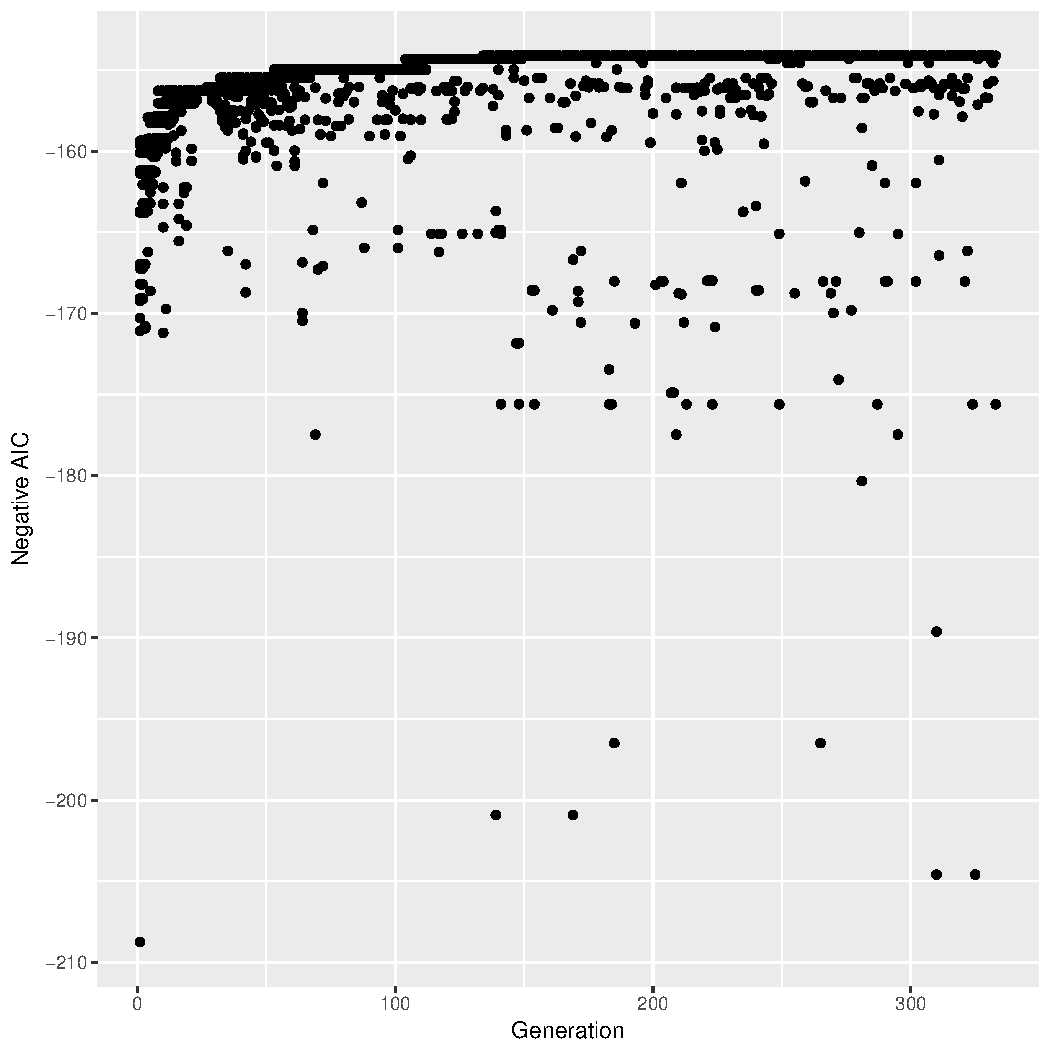
\includegraphics[width=\maxwidth]{figure/unnamed-chunk-1-2} 


\end{knitrout}
\end{document}
